\documentclass[letterpaper,12pt]{article}


\usepackage{listings}
\usepackage{color}
\usepackage{float}
\usepackage{graphicx}
\usepackage{subcaption}
% \usepackage{minted}

\definecolor{dkgreen}{rgb}{0,0.6,0}
\definecolor{gray}{rgb}{0.5,0.5,0.5}
\definecolor{mauve}{rgb}{0.58,0,0.82}



\lstset{frame=tb,
  language=C,
  aboveskip=3mm,
  belowskip=3mm,
  showstringspaces=false,
  columns=flexible,
  basicstyle={\small\ttfamily},
  numbers=none,
  numberstyle=\tiny\color{gray},
  keywordstyle=\color{blue},
  commentstyle=\color{dkgreen},
  stringstyle=\color{mauve},
  breaklines=true,
  breakatwhitespace=true,
  tabsize=3
}


\usepackage{tabularx} % extra features for tabular environment
\usepackage{amsmath}  % improve math presentation
\usepackage{graphicx} % takes care of graphic including machinery
\usepackage[margin=1in,letterpaper]{geometry} % decreases margins
\usepackage{cite} % takes care of citations
\usepackage[final]{hyperref} % adds hyper links inside the generated pdf file
\hypersetup{
	colorlinks=true,       % false: boxed links; true: colored links
	linkcolor=blue,        % color of internal links
	citecolor=blue,        % color of links to bibliography
	filecolor=magenta,     % color of file links
	urlcolor=blue         
}
%\documentclass{article}
\usepackage[utf8]{inputenc}
\usepackage[greek,english]{babel}
\usepackage{alphabeta}

\begin{document}

\graphicspath{{../Lab2/plots/}{../Lab1/plot/}}

\title{Συστήματα Παράλληλης Επεξεργασίας}
\author{Ομάδα 6 \\
Βασίλειος Βρεττός - el18126, \\
Ανδρέας Βατίστας - el18020, \\
Αλέξανδρος Τσάφος - el18211\\}
\date{Σχολή Ηλεκτρολόγων Μηχανικών και Μηχανικών Υπολογιστών, Εθνικό Μετσόβιο Πολυτεχνείο}
\maketitle




\section{Άσκηση 1 - Εξοικείωση με το περιβάλλον προγραμματισμού}
Η συγκεκριμένη άσκηση είναι εισαγωγική με σκοπό την εξοικείωση μας με τα μηχανήματα του cslab στα οποία εκτελούμε τις εργασίες. Για να δοκιμάσουμε την κατανόησή μας, ζητήθηκε να παραλληλοποιήσουμε το Conway’s Game of Life, ένα απλό παιχνίδι το οποίο “παίζεται” πάνω σε ένα ταμπλό (στην δική μας περίπτωση, διαστάσεων N x N). Το παιχνίδι τρέχει για Κ γύρους (χρονικά διαστήματα). Το κάθε σημείο του ταμπλό έχει 2 καταστάσεις, είτε ζωντανό ή νεκρό. Οι 2 κύριοι κανόνες του παιχνιδιού είναι: \newline

1.	Αν ένα ζωντανό σημείο έχει περισσότερους από 3 γείτονες ή λιγότερους από 2, τότε γίνεται νεκρό στον επόμενο γύρο. Αν έχει ακριβώς 2 ή 3, παραμένει ζωντανό. 

2.	Αν ένα νεκρό σημείο έχει ακριβώς 3 γείτονες, γίνεται ζωντανό στον επόμενο γύρο \newline

Τρέχουμε το παραπάνω σενάριο για 1000 γενιές (γύρους) σε πίνακες διαστάσεων 64x64, 1024x1024 και 4096x4096. \newline

Ο κώδικας ο οποίος ζητείται να παραλληλοποιηθεί είναι ο εξής.


\begin{lstlisting}
for ( t = 0 ; t < T ; t++ ) {
        #pragma omp parallel for shared (previous, current) private (i,j,nbrs)
         for ( i = 1 ; i < N-1 ; i++ )
            for ( j = 1 ; j < N-1 ; j++ ) {
                nbrs = previous[i+1][j+1] + previous[i+1][j] + previous[i+1][j-1] \
                       + previous[i][j-1] + previous[i][j+1] \
                       + previous[i-1][j-1] + previous[i-1][j] + previous[i-1][j+1];
                if ( nbrs == 3 || ( previous[i][j]+nbrs ==3 ) )
                    current[i][j]=1;
                else
                    current[i][j]=0;
            }

        #ifdef OUTPUT
        print_to_pgm(current, N, t+1);
        #endif
        //Swap current array with previous array
        swap=current;
        current=previous;
        previous=swap;
    }
\end{lstlisting}



Το πρώτο for-loop, το οποίο είναι η αλλαγή των γενιών, δεν έχει νόημα να παραλληλοποιηθεί αφού χρειαζόμαστε την τιμή της προηγούμενης γενιάς για να υπολογίσουμε τις καταστάσεις των κελιών για την επόμενη γενιά.


Η δική μας προσθήκη στον κώδικα είναι η γραμμή.

\begin{lstlisting}
 #pragma omp parallel for shared (previous, current) private (i,j,nbrs)
\end{lstlisting}


Το συγκεκριμένο compiler directive (pragma) είναι χαρακτηριστικό του OpenMP. Είναι μια “οδηγία” προς τον μεταγλωττιστή η οποία του ζητάει να παραλληλοποιηθούν τα εσωτερικά for-loops με νήματα ορισμένα από ένα environmental variable. Στο συγκεκριμένο directive, επίσης ζητάμε:

1.	Οι δείκτες previous, current να μοιράζονται μεταξύ των νημάτων. Η διάσταση Ν μοιράζεται by default.

2.	Οι μεταβλητές i,j,nbrs να είναι ξεχωριστές για κάθε νήμα.
\newline

Την απόδοση του πολυνηματισμού θα εξετάσουμε με χρήση την μετρική του χρόνου, και κατά συνέπεια, του speedup $S=\frac{T_s}{T_p}$ . \newline

\begin{figure}[H]
    \centering
    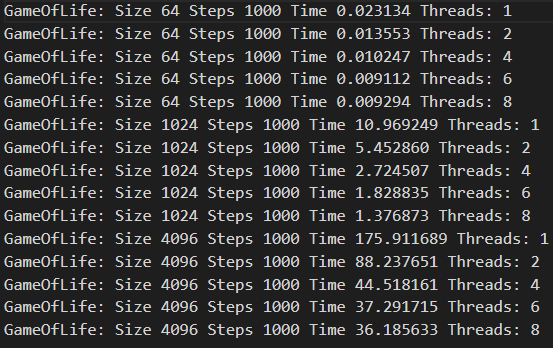
\includegraphics[scale=0.5]{/results.png}
    \caption{Έξοδος Game of Life}
    \label{fig:Έξοδος Game Of Life}
\end{figure}

\begin{figure}[H]
    \centering
    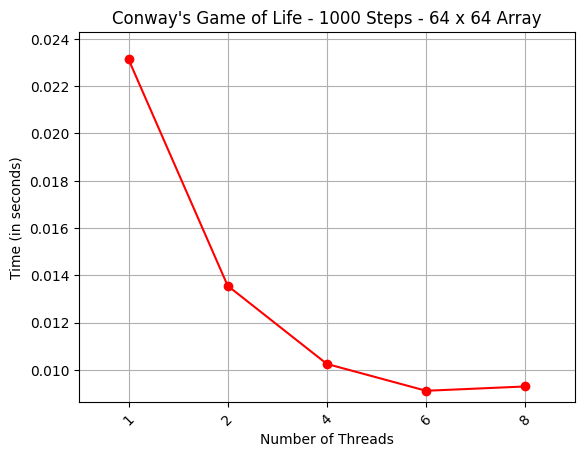
\includegraphics[scale=0.45]{/time_plots/time_64.png}
    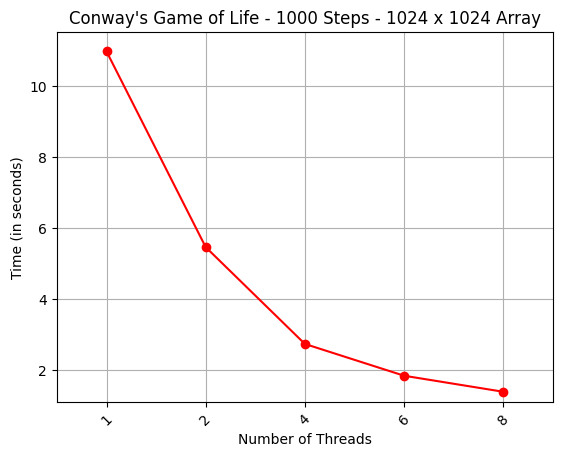
\includegraphics[scale=0.45]{/time_plots/time_1024.png}
    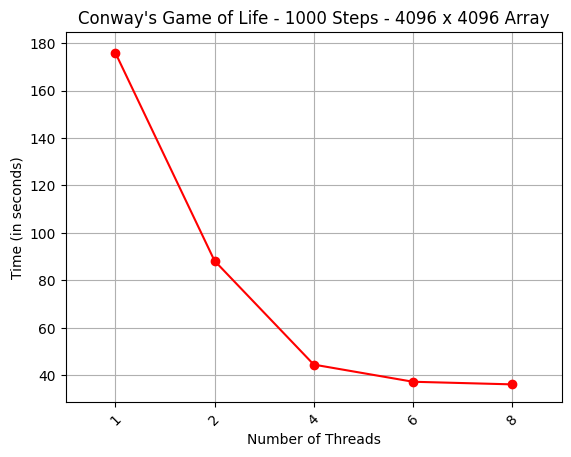
\includegraphics[scale=0.45]{/time_plots/time_4096.png}
    \caption{Χρόνος Εκτέλεσης Game of Life}
    \label{fig:Χρόνος Εκτέλεσης Game Of Life}
\end{figure}

\begin{figure}[H]
    \centering
    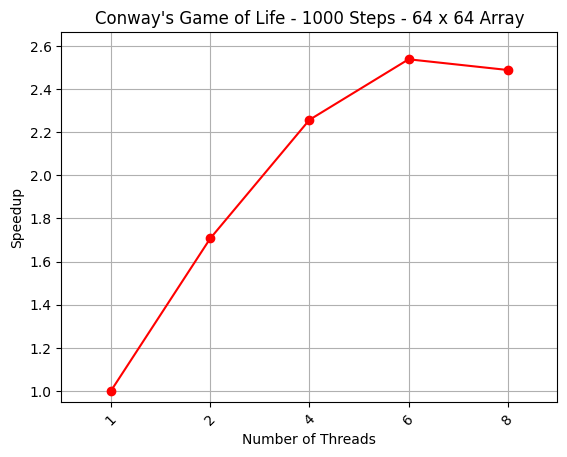
\includegraphics[scale=0.4]{/speedup_plots/speedup_64.png}
    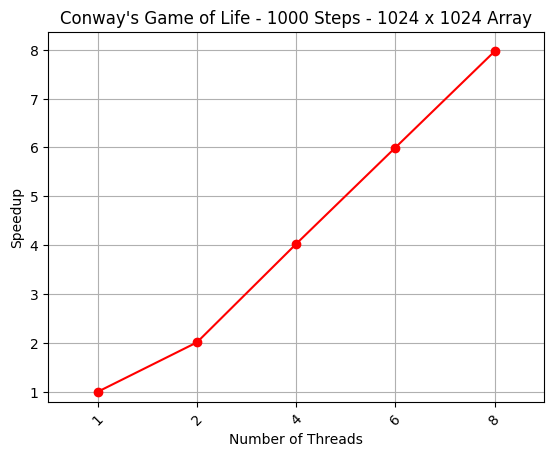
\includegraphics[scale=0.4]{/speedup_plots/speedup_1024.png}
    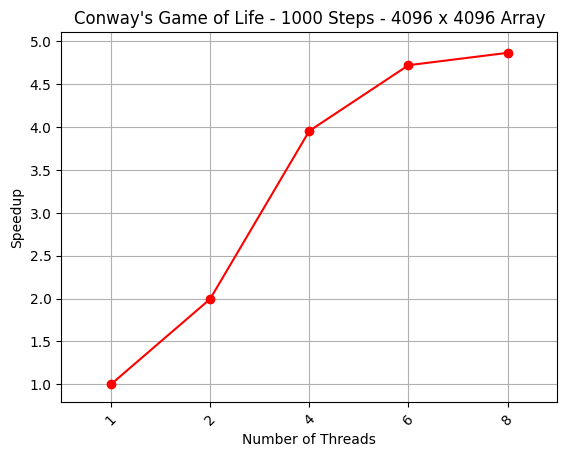
\includegraphics[scale=0.4]{/speedup_plots/speedup_4096.png}
    \caption{Speedup Game of Life}
    \label{fig:Speedup Game Of Life}
\end{figure}

\subsection*{Συμπεράσματα}
\subsubsection*{Για διαστάσεις 64x64}

Παρατηρούμε ότι η μείωση του χρόνου δεν είναι ακριβώς ανάλογη των αριθμών των νημάτων. Από 1 σε 2 νήματα ή από 2 σε 4 νήματα βλέπουμε σημαντική βελτίωση της απόδοσης. Η εναλλαγή από 4 σε 6 νήματα προσφέρει πολύ μικρότερη αύξηση απόδοσης. Τέλος, από 6 σε 8 νήματα παρατηρούμε \textbf{ΑΥΞΗΣΗ} του χρόνου εκτέλεσης (μηδαμινή). 

Η συγκεκριμένη αύξηση οφείλεται στο overhead που υπάρχει με την χρήση πολυνηματισμού σε μια διεργασία (γέννηση νημάτων, επικοινωνία κ.λ.π.). Ο συγκεκριμένος πίνακας είναι τόσο μικρός που η παραλληλοποίησή του περαιτέρω δεν βγάζει νόημα. Αν είχαμε την δυνατότητα να εξετάσουμε μεγαλύτερο αριθμό νημάτων, πολύ πιθανό να βλέπαμε περαιτέρω αύξηση του χρόνου εκτέλεσης
\subsubsection*{Για διαστάσεις 1024x1024}

Παρατηρούμε ότι το speedup τείνει να είναι πλήρως γραμμικό. Ο χρόνος υποδιπλασιάζεται με κάθε διπλασιασμό νημάτων. Το συγκεκριμένο ταμπλό φαίνεται ιδανικό για παραλληλοποίηση. Η επικοινωνία μεταξύ νημάτων δεν περιορίζει την απόδοσή τους
\subsubsection*{Για διαστάσεις 4096x4096}

Στους πρώτους 2 διπλασιασμούς των threads, βλέπουμε γραμμική μείωση του χρόνου (υποδιπλασιασμός) και κατά συνέπεια γραμμική αύξηση του speedup. Η λογική αυτή σταματάει να ισχύει για περαιτέρω αύξηση των νημάτων. Το συγκεκριμένο φαινόμενο δικαιολογείται από την ύπαρξη μεγάλου φόρτου (συμφόρησης) στον διάδρομο μνήμης. Υπάρχει συχνός διαμοιρασμός δεδομένων μεταξύ νημάτων καθώς αυξάνονται οι τιμές που πρέπει να ελεγχθούν για να υπολογιστούν οι γείτονες.


\section{Άσκηση 2 - Παραλληλοποίηση και βελτιστοποίηση αλγορίθμων σε αρχιτεκτονικές κοινής μνήμης}

Στην συγκεκριμένη άσκηση, σκοπός είναι η παραλληλοποίηση 2 διαφορετικών εκδόσεων των αλγορίθμων K-means και Floyd-Warshall.
% Συμπλήρωσε πραγματα...

\subsection{Αλγόριθμος K-means}

Ο αλγόριθμος k-means διαχωρίζει N αντικείμενα σε k μη επικαλυπτόμενες ομάδες. Ο παρακάτω ψευδοκώδικας περιγράφει τον αλγόριθμο.

\begin{lstlisting}
until convergence (or fixed loops)
    for each object
        find nearest cluster
    for each cluster
        calculate new cluster center coordinates.
\end{lstlisting}

Στο συγκεκριμένο πρόβλημα μελετάμε 2 διαφορετικές εκδόσεις. Στην 1η, ο πίνακας των συντεταγμένων μοιράζεται από τα νήματα (shared cluster).
Στην 2η υλοποίηση, δίνουμε στο κάθε νήμα μια τοπική έκδοση του πίνακα. Έτσι, τα νήματα μπορούν να κάνουν πράξεις
χωρίς να υπάρχουν προβλήματα διαμοιρασμού (cache invalidation e.t.c.). Στο τέλος, κάθε νήμα ενημερώνει το
master thread με τα δικα του αποτελέσματα (reduction).

\subsubsection{K-means - Shared Clusters}

Το μειονέκτημα της συγκεκριμένης υλοποίησης είναι ότι εφόσον λειτουργούμε πάνω σε διαμοιραζόμενα δεδομένα, υπάρχει
ανάγκη η ανανέωση των shared variables \textbf{newClusterSize} και \textbf{newClusters} να γίνεται ατομικά.

Τα κλειδώματα για την ανανέωση των μεταλητών έγινε με την χρήση του \textbf{atomic} pragma.

Το πρόγραμμα λήγει για συγκεκριμένα iterations ή μέχρι να συγκλίνει. Τα παρακάτω δεδομένα είναι για τον συνδυασμό
\{Size, Coords, Clusters, Loops\} = \{256, 16, 16, 10\}.

\begin{lstlisting}
    #pragma omp parallel for default(shared) shared(newClusterSize, newClusters) private(i, j, index)
    for (i=0; i<numObjs; i++){
    /*
     *
     */
    #pragma omp atomic
    newClusterSize[index]++;
    /*
     *
     */
     #pragma omp atomic
     newClusters[index*numCoords + j] += objects[i*numCoords + j];
    }
\end{lstlisting}

\begin{figure}[H]
    \centering
    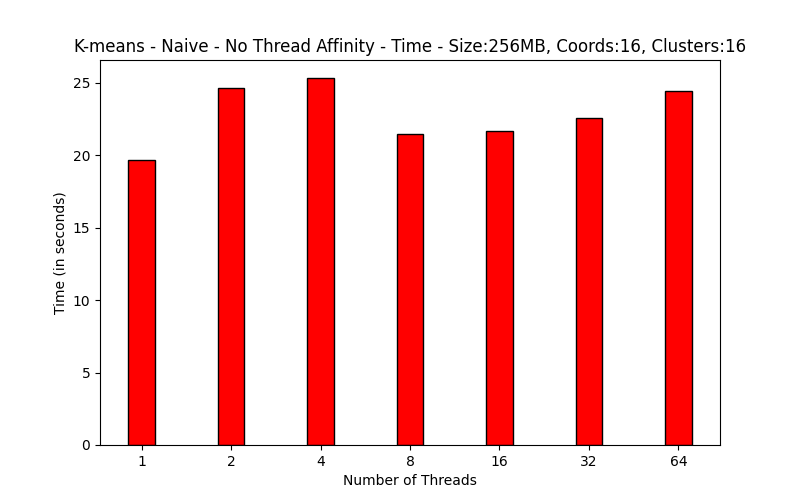
\includegraphics[scale=0.40]{/kmeansNaivePlots/kmeans_naive_no_affinity.png}
    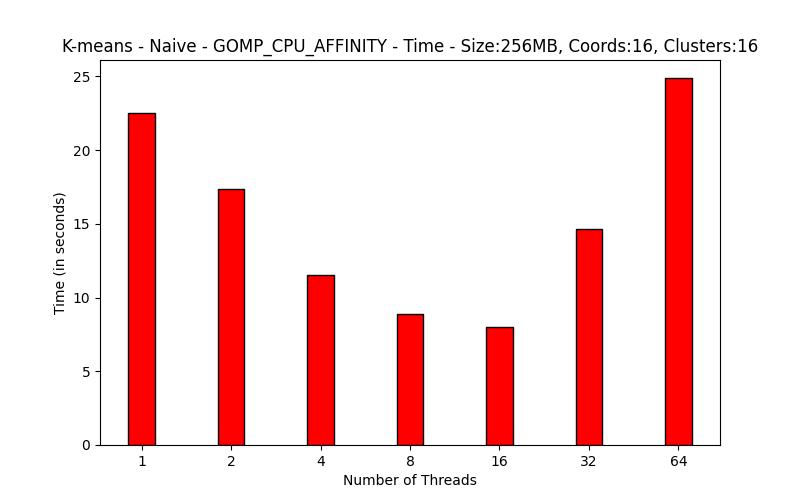
\includegraphics[scale=0.40]{/kmeansNaivePlots/kmeans_naive_gomp_cpu_affinity.png}
    \caption{Χρόνος Εκτέλεσης K-Means Naive}
    \label{fig:Χρόνος Εκτέλεσης K-Means Naive}
\end{figure}

\begin{figure}[H]
    \centering
    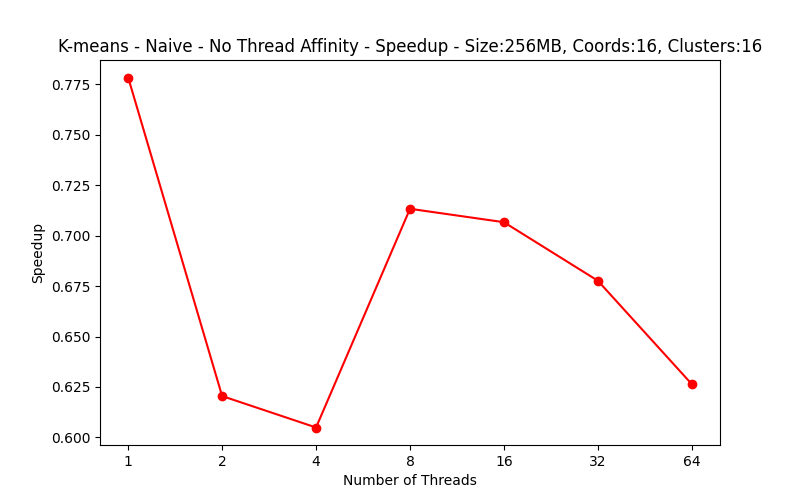
\includegraphics[scale=0.40]{/kmeansNaivePlots/kmeans_naive_no_affinity_speedup.png}
    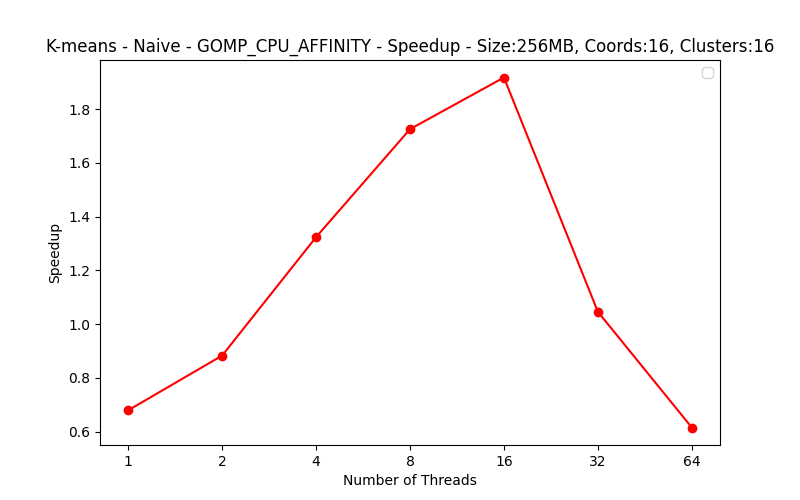
\includegraphics[scale=0.40]{/kmeansNaivePlots/kmeans_naive_gomp_cpu_affinity_speedup.png}
    \caption{Speedup K-Means Naive}
    \label{fig:Speedup K-Means Naive}
\end{figure}

\textbf{Σημείωση:} Για το speedup θεωρούμε σειριακό χρόνο εκτέλεσης την έκδοση ΧΩΡΙΣ κλειδώματα.
Εδώ το speedup με 1 νήμα είναι μικρότερο της μονάδας γιατί έχουμε κλειδώματα.
\vspace{4pt}

Το άμεσο συμπέρασμα είναι ότι το πρόγραμμα δεν βελτιώνεται με χρήση παραπάνω νημάτων. Συγκεκριμένα, 
η αύξηση των διαθέσιμων νημάτων αυξάνει τον χρόνο εκτέλεσης. 
% Προσθεσε συμπερασματα

Σαν προσπάθεια να βελτιώσουμε τα αποτελέσματα, χρησιμοποιήσαμε την μεταβλητή περιβάλλοντος GOMP\_CPU\_AFFINITY.
Η λειτουργία αυτής της μεταβλήτης είναι ότι προσδένει τα "λογικά" νήματα σε hardware νήματα των επεξεργαστών βάσει μιας ακολουθίας.
Γνωρίζοντας ότι οι επεξεργαστές του Sandman θεωρούν ότι π.χ. στο Physical Core 0 υπάρχουν τα Logical Cores (0,32),
επιλέξαμε τα νήματα να προσδένονται ακολουθιακά στους φυσικούς πυρήνες των επεξεργαστών.

Παρατηρήσαμε βελτίωση των χρόνων για τα πρώτα 32 νήματα. Φυσικό ήταν να μην βελτιωθεί η κατάσταση για τα 64 νήματα.
% Πες κιαλα


\subsubsection{K-means - Copied Clusters and Reduce}

\subsection{Αλγόριθμος Floyd-Warshall}

Έστω πίνακας "γειτνίασης" Α. Ο κώδικας σε C για τον αλγόριθμο Floyd-Warshall είναι ο εξής:

\begin{lstlisting}
    for (k=0; k<N; k++)
        for (i=0; i<N; i++)
           for (j=0; j<N; j++)
                A[i][j] = min(A[i][j], A[i][k]+A[k][j]);
\end{lstlisting}

Το κομμάτι το οποίο μπορεί να παραλληλοποιηθεί είναι οι 2 εσωτερικά-φωλιασμένοι βρόγχοι.

\subsubsection{Floyd-Warshall - Standard Edition}
Η standard έκδοση του αλγορίθμου (σε C με OpenMP) είναι ως εξής:

\begin{lstlisting}
    for(k=0;k<N;k++)
        #pragma omp parallel for shared(A) private(i,j)
        for(i=0; i<N; i++)
            for(j=0; j<N; j++)
                A[i][j]=min(A[i][j], A[i][k] + A[k][j]);
\end{lstlisting}

\begin{figure}[H]
    \centering
    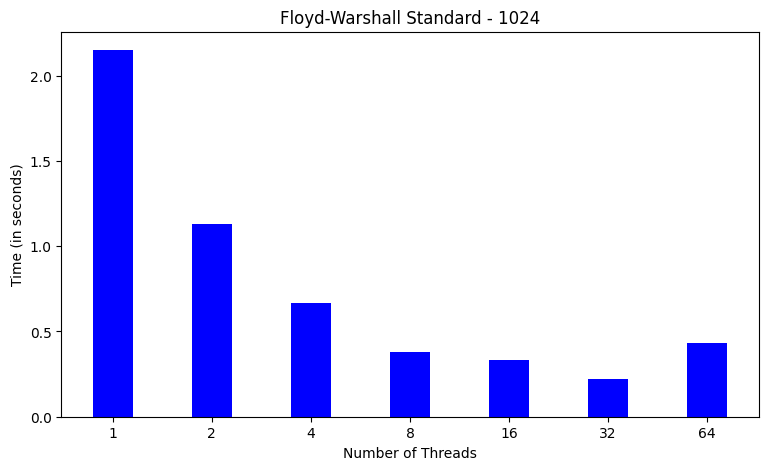
\includegraphics[scale=0.4]{/fwStandardPlots/fw_standard_1024.png}
    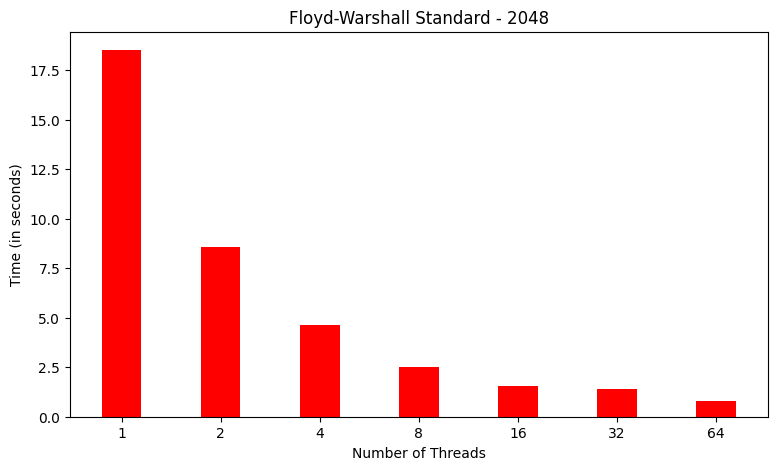
\includegraphics[scale=0.4]{/fwStandardPlots/fw_standard_2048.png}
    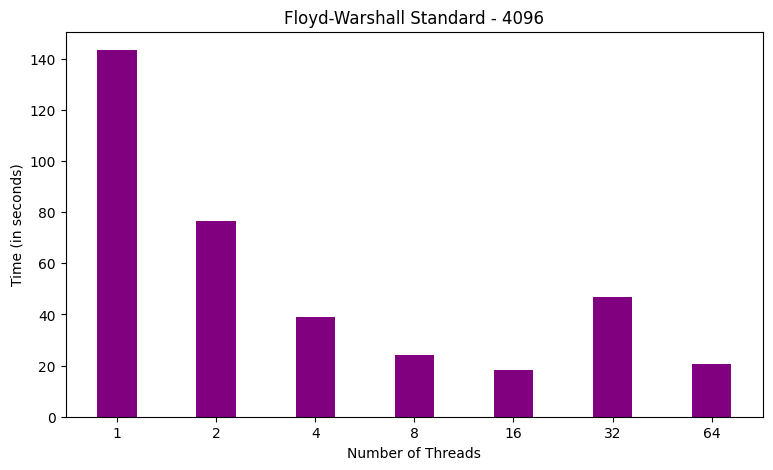
\includegraphics[scale=0.4]{/fwStandardPlots/fw_standard_4096.png}
    \caption{Χρόνος Εκτέλεσης FW Standard}
    \label{fig:Χρόνος Εκτέλεσης FW Standard}
\end{figure}

\begin{figure}[H]
    \centering
    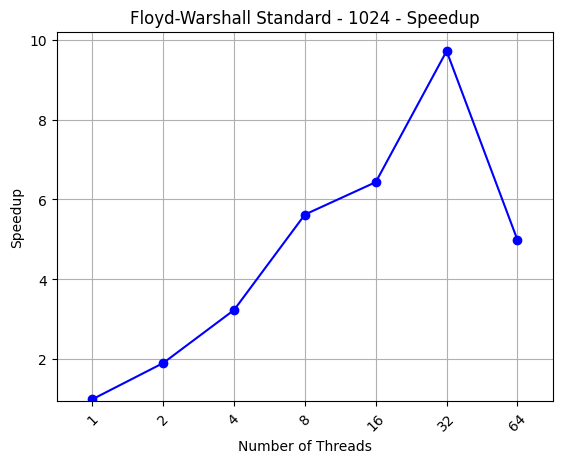
\includegraphics[scale=0.50]{/fwStandardPlots/fw_speedup1024.png}
    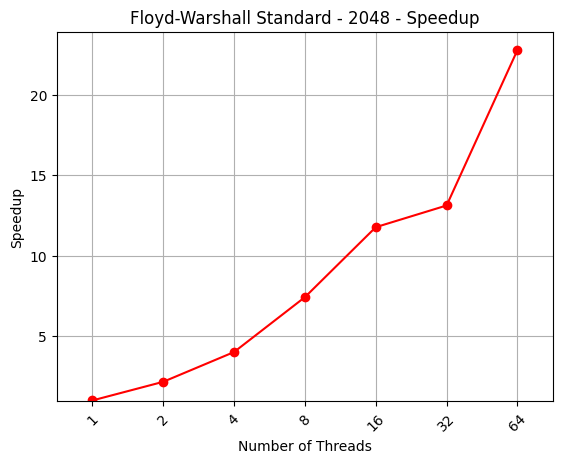
\includegraphics[scale=0.50]{/fwStandardPlots/fw_speedup2048.png}
    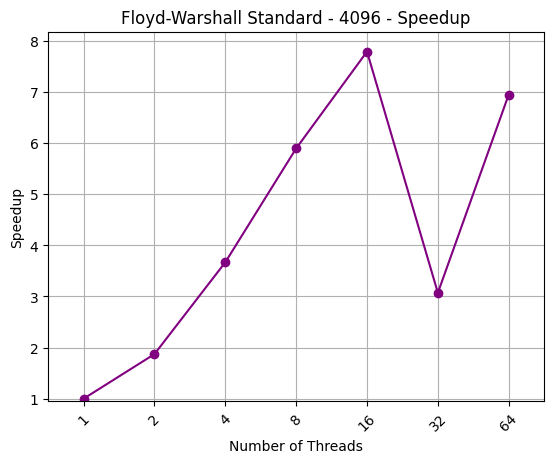
\includegraphics[scale=0.50]{/fwStandardPlots/fw_speedup4096.png}
    \caption{Speedup FW Standard}
    \label{fig:Speedup FW Standard}
\end{figure}

Παρατηρούμε ότι τα συμπεράσματα πέρι κλιμάκωσης είναι ολόιδια με το πρόβλημα του Game Of Life.
Για μικρούς πίνακες, υπάρχει μεγάλη δυνατότητα για κλιμάκωση, αλλά αυξάνοτας τα νήματα, η το overhead
που εισάγεται λόγω της επικοινωνίας μεταξύ τους περιορίζει την αύξηση της απόδοσης

Για μεσαίους πίνακες, οι οποίοι χωράνε στην cache των πυρήνων, έχουμε ακόμα μεγαλύτερη δυνατότητα για κλιμάκωση.

Για μεγάλους πίνακες, το πρόβλημα γίνεται πιο περίπλοκο καθώς πλέον δεν χωράει ο πίνακας στις cache μνήμες του επεξεργαστή.
Αυξάνονται οι ανάγκες για μεταφορά cache lines. Άρα πλέον το πρόβλημα είναι memory bound. 

\subsubsection{Floyd-Warshall - Recursive/Task Based}

Το νόημα της συγκεκριμένης έκδοσης του αλγορίθμου είναι να τρέχει αναδρομικά μέχρι να συναντήσει πίνακα
μεγέθους, επιλεγμένο από εμας, βολικό για τον επεξεργαστή. Το μέγεθος αυτό ονομάζουμε block size. Δηλαδή, προσπαθούμε να χωρέσουμε ολόκληρο τον
πίνακα στην cache. Παρακάτω παρουσιάζουμε το task graph της συνάρτησης αυτής για την πρώτη φορά που καλείται.

\begin{figure}[H]
    \centering
    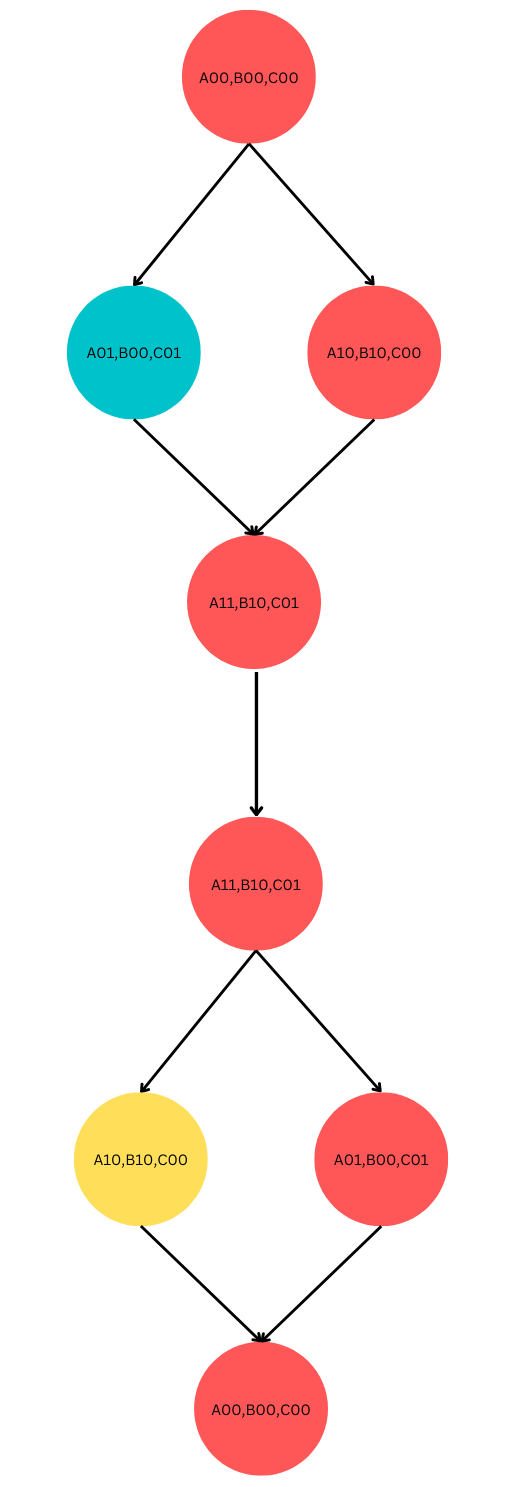
\includegraphics[scale=0.25]{/taskgraph.png}
    \caption{FW Recursive Task Graph - 1st iteration}
    \label{fig:FW Recursive Task Graph}
\end{figure}

Η παραλληλοποίηση αυτής της έκδοσης γίνεται με χρήση task, ώστε να μπορεί να είναι αναδρομική.
Η OpenMP προσφέρει αυτή την δυνατότητα με την χρήση του

\begin{lstlisting}
#pragma omp task
\end{lstlisting}



\begin{figure}[H]
    \centering
    \begin{subfigure}[b]{0.45\linewidth}
        \includegraphics[scale=0.42]{/fwTaskPlots/fw_tasks_1024.png}
        \caption{FW Recursive Size 1024}
    \end{subfigure}
    \begin{subfigure}[b]{0.45\linewidth}
        \includegraphics[scale=0.42]{/fwTaskPlots/fw_tasks_2048.png}
        \caption{FW Recursive Size 2048}
    \end{subfigure}
    \begin{subfigure}[b]{0.5\linewidth}
        \includegraphics[scale=0.42]{/fwTaskPlots/fw_tasks_4096.png}
        \caption{FW Recursive Size 4096}
    \end{subfigure}
    \caption{Χρόνος Εκτέλεσης FW Recursive}
    \label{fig:Χρόνος Εκτέλεσης FW Recursive}
\end{figure}

\begin{figure}[H]
    \centering
    \begin{subfigure}[b]{0.48\linewidth}
        \includegraphics[scale=0.42]{/fwTaskPlots/fw_tasks_speedup_1024.png}
        \caption{FW Recursive Size 1024}
    \end{subfigure}
    \begin{subfigure}[b]{0.48\linewidth}
        \includegraphics[scale=0.42]{/fwTaskPlots/fw_tasks_speedup_2048.png}
        \caption{FW Recursive Size 2048}
    \end{subfigure}
    \begin{subfigure}[b]{0.5\linewidth}
        \includegraphics[scale=0.42]{/fwTaskPlots/fw_tasks_speedup_4096.png}
        \caption{FW Recursive - Size 4096 - Speedup}
    \end{subfigure}
    \caption{Speedup FW Recursive}
    \label{fig:Speedup FW Recursive}
\end{figure}

Η πρώτη παρατήρηση είναι ότι το speedup δεν ξεπερνάει το 1.4. Σύμφωνα και με το task graph, η μέγιστη
παραλληλοποίησή γίνεται με 2 νήματα σε κάθε επίπεδο αναδρομής. Ως προεπιλογή, το OpenMP \textbf{ΔΕΝ}
επιτρέπει φωλιασμένη παραλληλοποίηση. Όταν ένα νήμα εισέρχεται σε παράλληλη περιοχή μέσα σε άλλη παράλληλη περιοχή,
τότε δεν καλεί παραπάνω νήματα για την εκτέλεση αυτής της περιοχής. Άρα υπάρχουν περιοχές στο πρόγραμμα που εκτελούνται
με το πολύ 1 εργάτη.

Η λύση για το παραπάνω είναι να αλλάξουμε την συμπεριφορά του OpenMP. Γίνεται να προσπεράσουμε αυτόν τον περιορισμό
θέτοντας ένα environmental variable, το \textbf{OMP\_NESTED}
σε \textbf{TRUE}.

Η λύση αυτή δεν επαρκεί καθώς μετά μπορεί να επιφέρει αντίθετα αποτελέσματα από τα επιθυμητά.
Επιτρέποντας την εκτέλεση φωλιασμένων παράλληλων περιοχών, υπάρχει ο κίνδυνος να καλέσουμε πολλά νήματα για την
δημιουργία των task αλλά να μην υπάρχουν διαθέσιμα νήματα για την ίδια την εκτέλεση των πράξεων.

Χρειάζονται περαιτέρω περιορισμοί. Αυτοί δίνονται από το OpenMP με την μορφή μεταβλητών
περιβάλλοντος.
\\
Οι \textbf{SUNW\_MP\_MAX\_POOL\_THREADS} και 
\textbf{SUNW\_MP\_MAX\_NESTED\_LEVELS} περιορίζουν τον αριθμό των διαθέσιμων
νημάτων/δούλων (δηλαδή όλων εκτός του νήματος αφέντη) και το μέγιστο βάθος που επιτρέπονται από τα νήματα να καλούν
άλλα νήματα αντίστοιχα.

Εφαρμόζοντας τα παραπάνω, βγάζουμε τα παρακάτω αποτελέσματα:

\begin{figure}[H]
    \centering
    \begin{subfigure}[b]{0.45\linewidth}
        \includegraphics[scale=0.42]{/fwTaskNestedPlots/fw_tasks_1024.png}
        \caption{FW Recursive + Nested Size 1024}
    \end{subfigure}
    \begin{subfigure}[b]{0.45\linewidth}
        \includegraphics[scale=0.42]{/fwTaskNestedPlots/fw_tasks_2048.png}
        \caption{FW Recursive + Nested Size 2048}
    \end{subfigure}
    \begin{subfigure}[b]{0.5\linewidth}
        \includegraphics[scale=0.42]{/fwTaskNestedPlots/fw_tasks_4096.png}
        \caption{FW Recursive + Nested Size 4096}
    \end{subfigure}
    \caption{Χρόνος Εκτέλεσης FW Recursive/Nested}
    \label{fig:Χρόνος Εκτέλεσης FW Recursive/Nested}
\end{figure}

\begin{figure}[H]
    \centering
    \begin{subfigure}[b]{0.48\linewidth}
        \includegraphics[scale=0.42]{/fwTaskNestedPlots/fw_tasks_speedup_1024.png}
        \caption{FW Recursive - Size 1024 - Speedup}
    \end{subfigure}
    \begin{subfigure}[b]{0.48\linewidth}
        \includegraphics[scale=0.42]{/fwTaskNestedPlots/fw_tasks_speedup_2048.png}
        \caption{FW Recursive - Size 2048 - Speedup}
    \end{subfigure}
    \begin{subfigure}[b]{0.5\linewidth}
        \includegraphics[scale=0.42]{/fwTaskNestedPlots/fw_tasks_speedup_4096.png}
        \caption{FW Recursive - Size 4096 - Speedup}
    \end{subfigure}
    \caption{Speedup FW Recursive/Nested}
    \label{fig:Speedup FW Recursive/Nested}
\end{figure}




\subsubsection{Floyd-Warshall - Tiled}

Στην συγκεκριμένη έκδοση,

\begin{figure}[H]
    \centering
    \begin{subfigure}[b]{0.48\linewidth}
        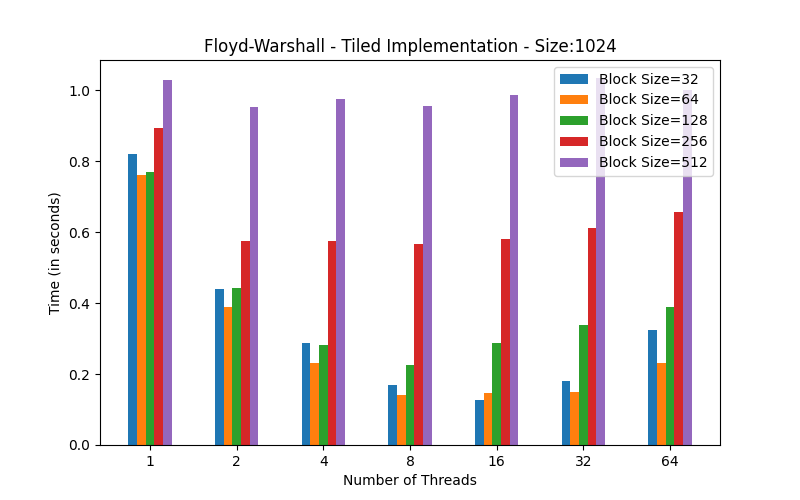
\includegraphics[scale=0.42]{/fwTiledPlots/fw_tiles_1024.png}
        \caption{FW Tiled - Size 1024}
    \end{subfigure}
    \begin{subfigure}[b]{0.48\linewidth}
        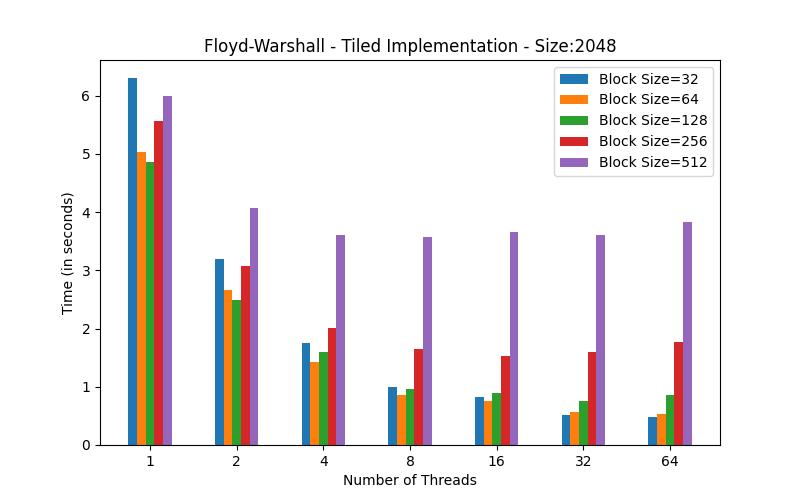
\includegraphics[scale=0.42]{/fwTiledPlots/fw_tiles_2048.png}
        \caption{FW Tiled - Size 2048}
    \end{subfigure}
    \begin{subfigure}[b]{0.5\linewidth}
        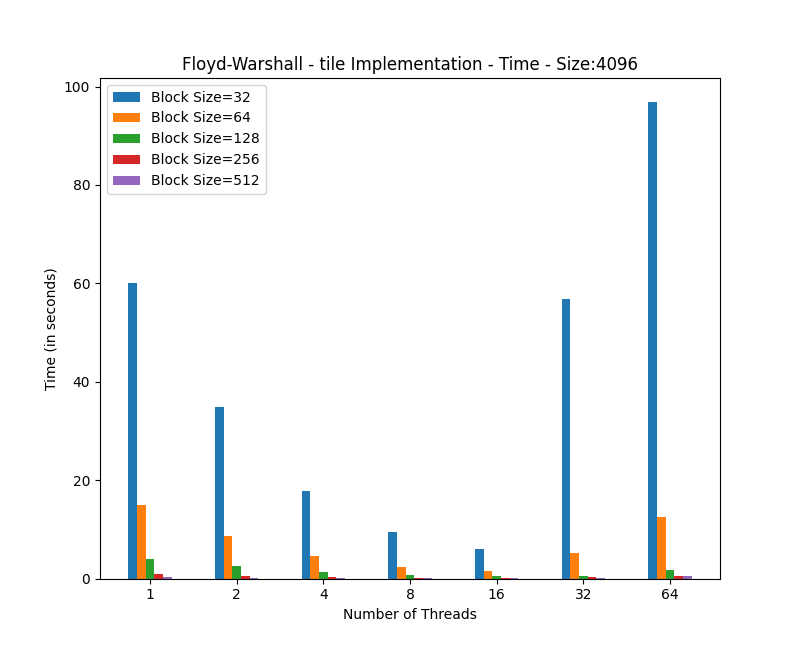
\includegraphics[scale=0.42]{/fwTiledPlots/fw_tiles_4096.png}
        \caption{FW Tiled - Size 4096}
    \end{subfigure}
    \caption{Χρόνος Εκτέλεσης FW Tiled}
    \label{fig:Χρόνος Εκτέλεσης FW Tiled}
\end{figure}

\begin{figure}[H]
    \centering
    \begin{subfigure}[b]{0.48\linewidth}
        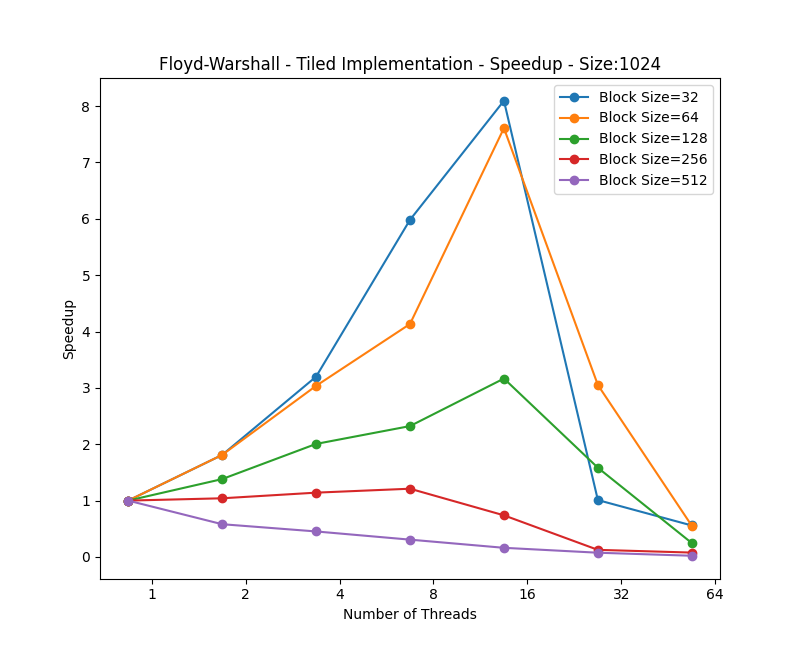
\includegraphics[scale=0.42]{/fwTiledPlots/fw_tiles_speedup_1024.png}
        \caption{FW Tiled - Size 1024 - Speedup}
    \end{subfigure}
    \begin{subfigure}[b]{0.48\linewidth}
        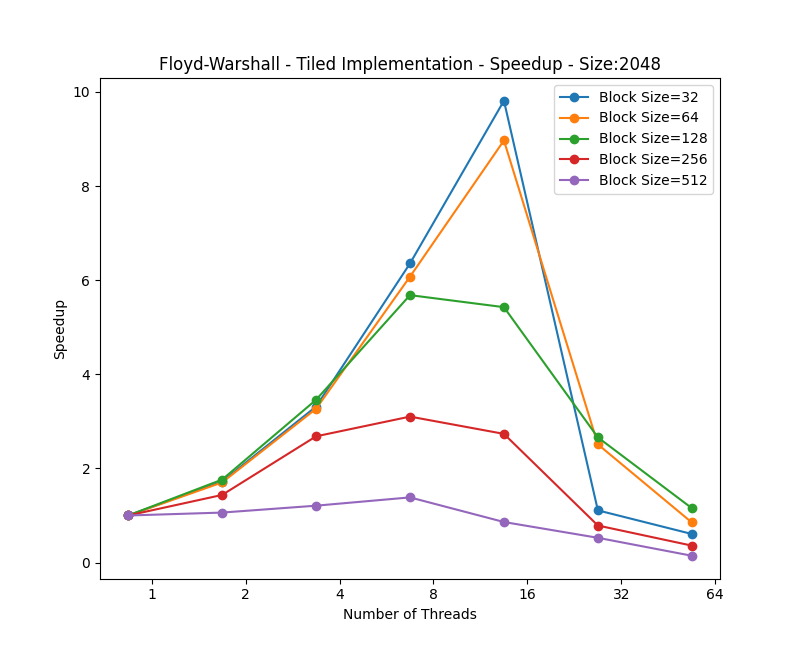
\includegraphics[scale=0.42]{/fwTiledPlots/fw_tiles_speedup_2048.png}
        \caption{FW Tiled - Size 2048 - Speedup}
    \end{subfigure}
    \begin{subfigure}[b]{0.5\linewidth}
        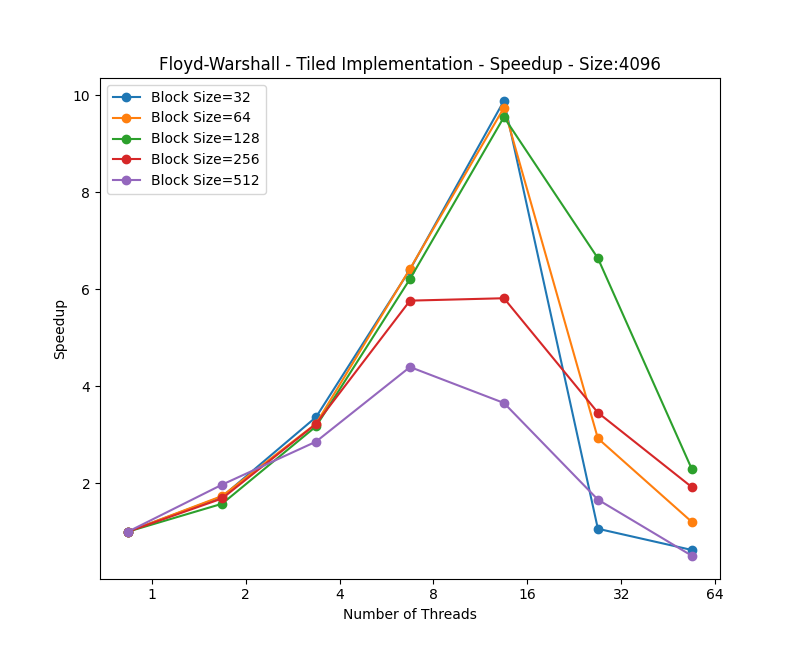
\includegraphics[scale=0.42]{/fwTiledPlots/fw_tiles_speedup_4096.png}
        \caption{FW Tiled - Size 4096 - Speedup}
    \end{subfigure}
    \caption{Speedup FW Tiled}
    \label{fig:Speedup FW Tiled}
\end{figure}


\end{document}